\section{联邦学习算法关于子节点训练参与率的鲁棒性的数值评测}
\addcontentsline{toe}{section}{{\thesection\ \ Numerical Evaluation of the Robustness of Federated Learning Algorithms on the Participation Rate of the Clients}\numberline\,}
\label{sec:chap6-sample}

% almost finished

上一节对几种典型的联邦学习算法的数值效果进行了比较,我们发现\texttt{FedProx}, \texttt{ProxSkip}, \texttt{FedSplit}等几种算法对于子节点训练参与率这一指标比较敏感。在本节,我们将对比这几种算法在子节点训练参与率分别为$10\%, 30\%, 70\%, 100\%$下,在数据集\texttt{FedProxFEMNIST}的测试集上的准确率曲线以及损失曲线。同时,我们将\texttt{IFCA}算法作为对照,参与比较。相关的曲线绘制在了图\ref{fig:compare-sample-ratio}~中。

\begin{figure}[H]
\centering
\begin{subfigure}{.5\textwidth}
  \centering
  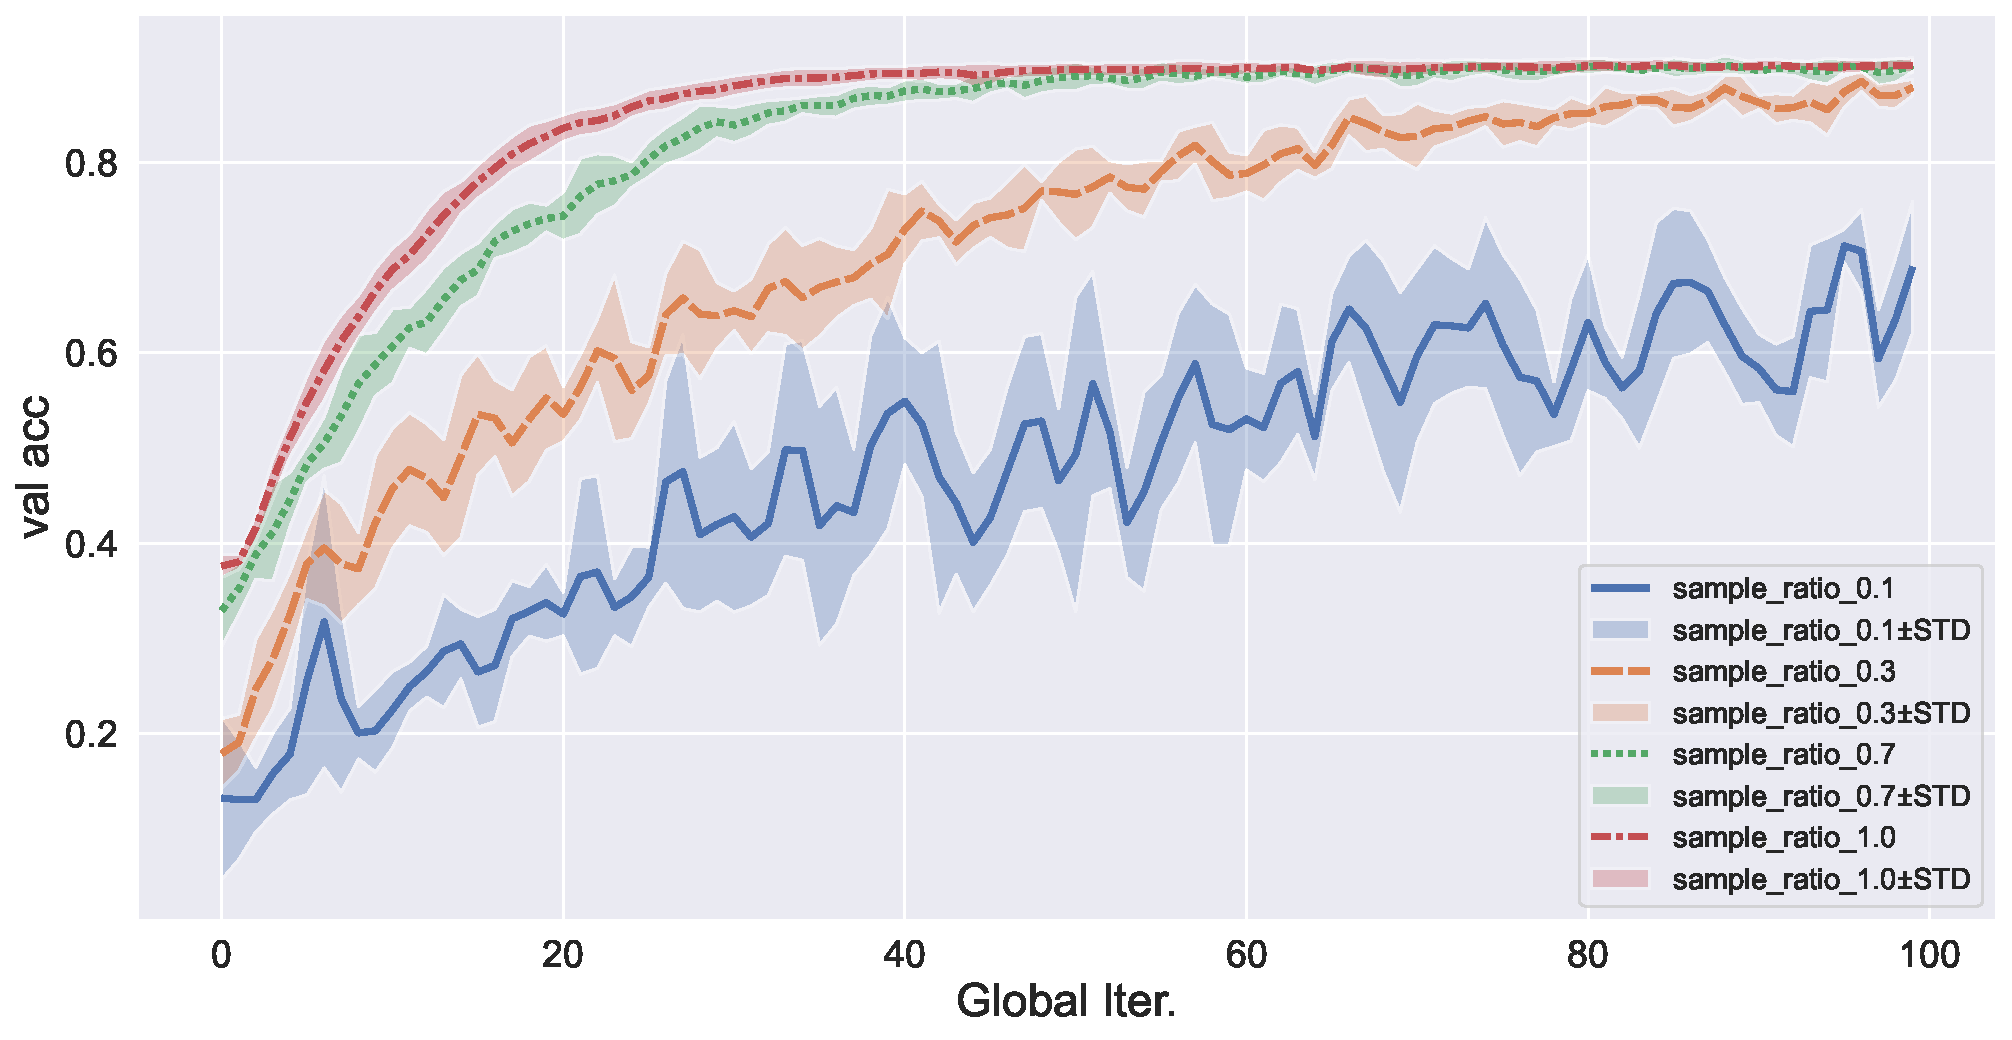
\includegraphics[width=.95\linewidth]{figures/fedprox-compare-sample-ratio-val-acc.pdf}
  \caption{\texttt{FedProx}算法在不同的子节点训练参与率下测试集上准确率曲线}
  \label{fig:fedprox-compare-sample-ratio-val-acc}
\end{subfigure}%
\begin{subfigure}{.5\textwidth}
  \centering
  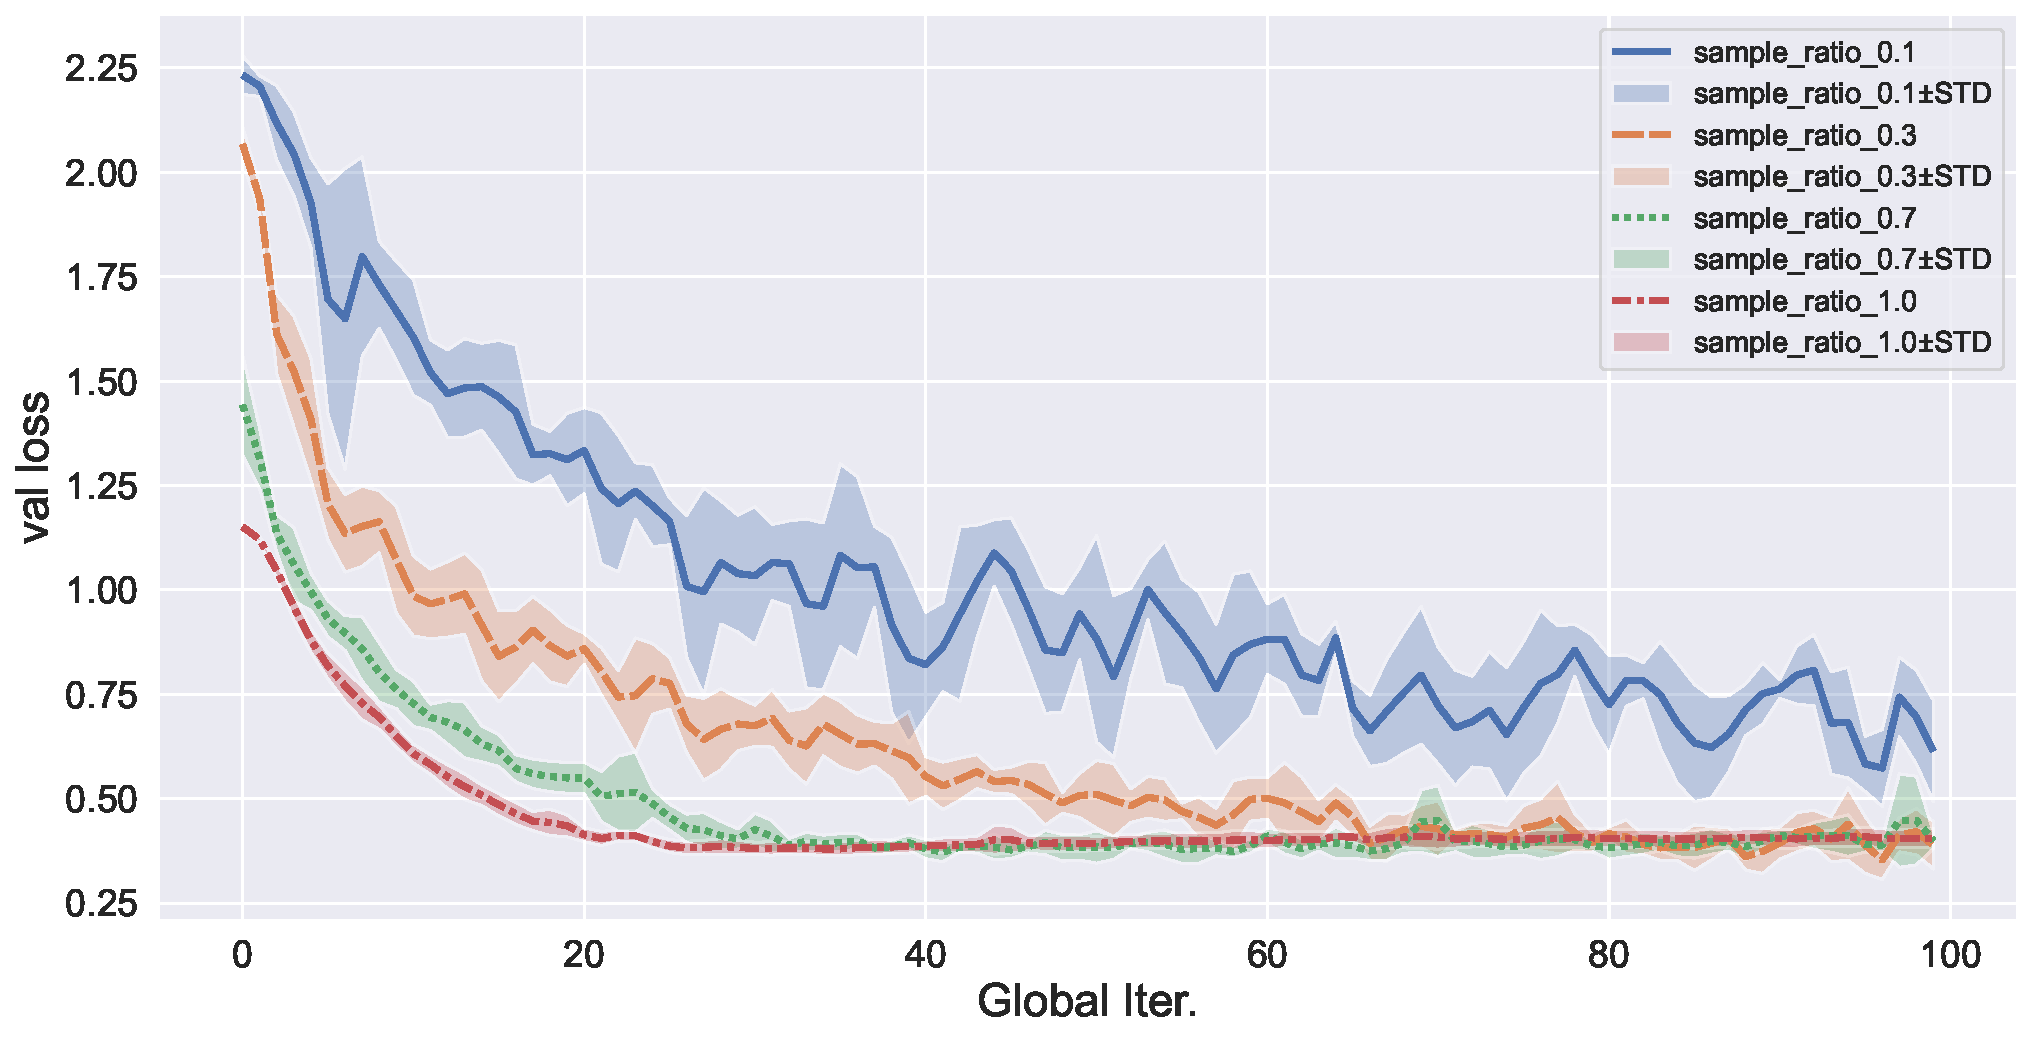
\includegraphics[width=.95\linewidth]{figures/fedprox-compare-sample-ratio-val-loss.pdf}
  \caption{\texttt{FedProx}算法在不同的子节点训练参与率下测试集上损失曲线}
  \label{fig:fedprox-compare-sample-ratio-val-loss}
\end{subfigure}
\begin{subfigure}{.5\textwidth}
  \centering
  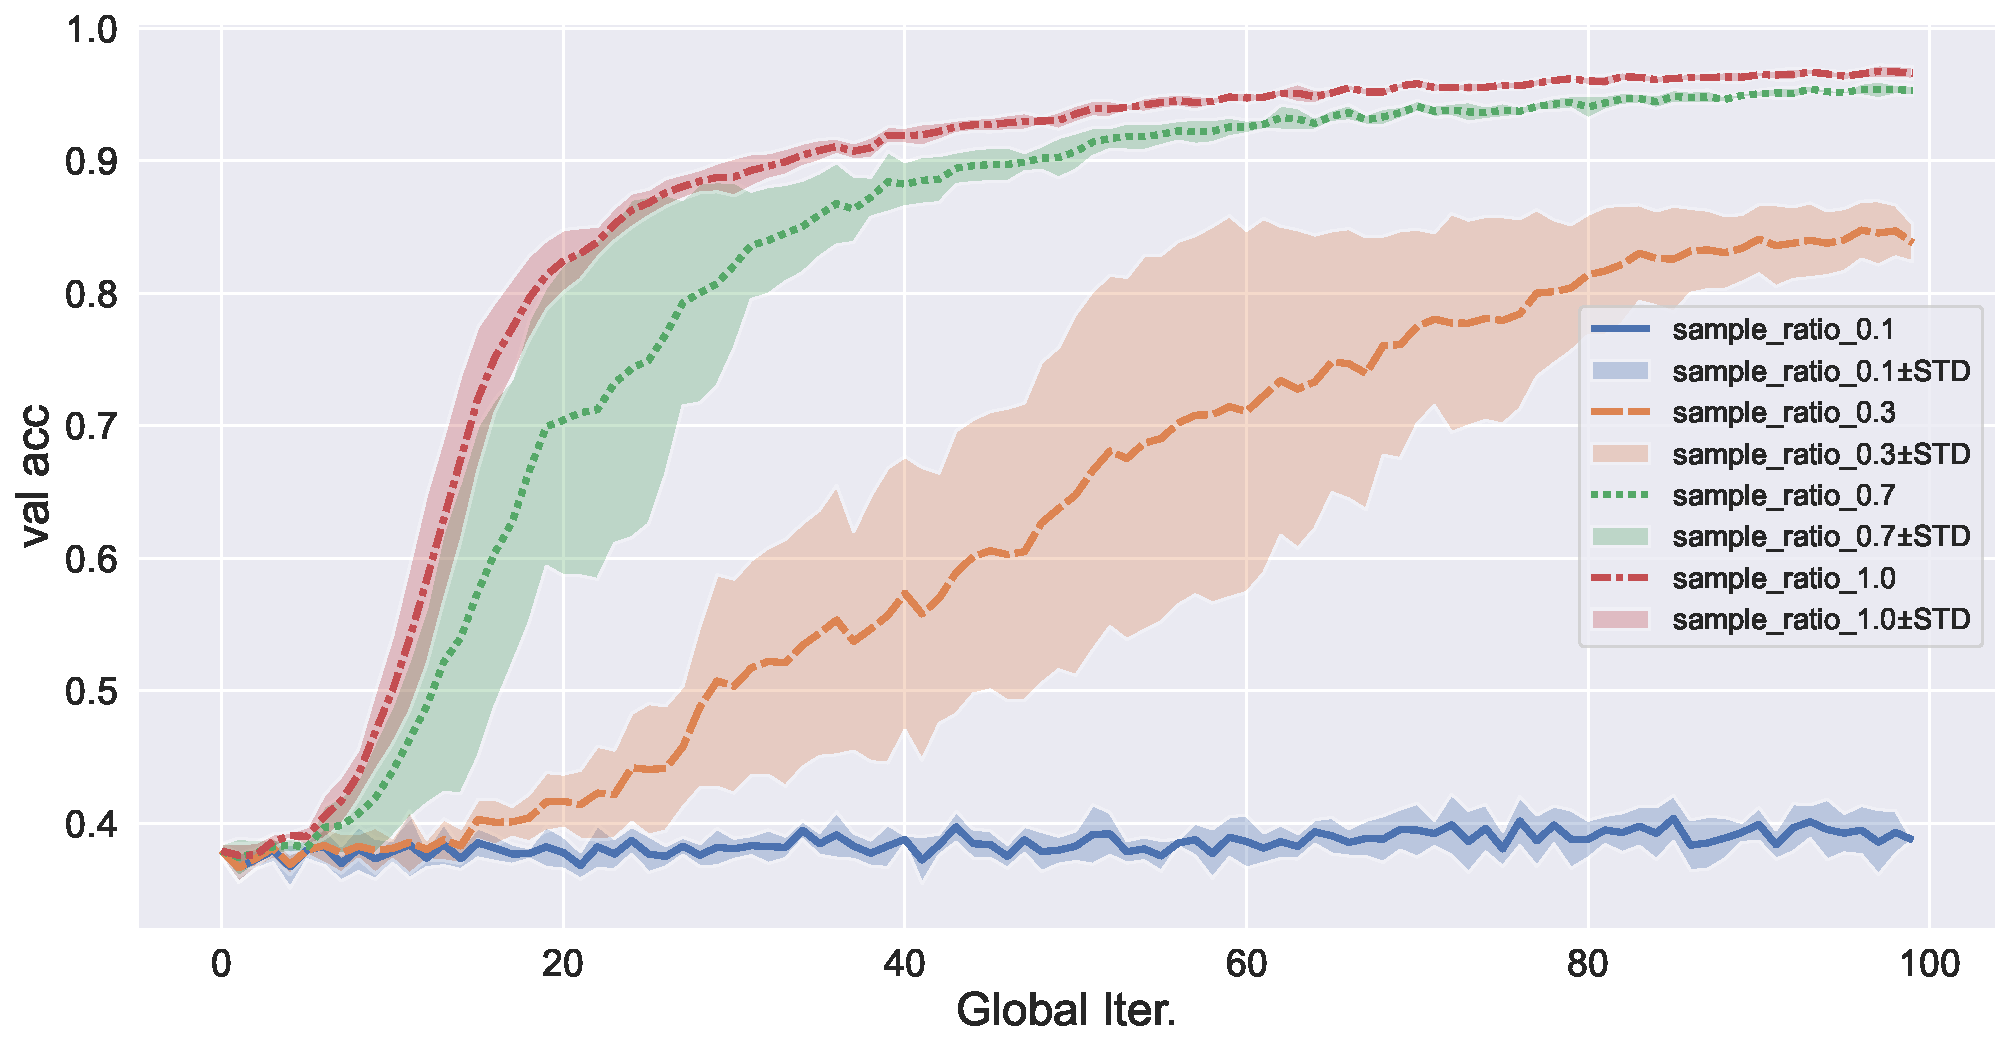
\includegraphics[width=.95\linewidth]{figures/proxskip-compare-sample-ratio-val-acc.pdf}
  \caption{\texttt{ProxSkip}算法在不同的子节点训练参与率下测试集上准确率曲线}
  \label{fig:proxskip-compare-sample-ratio-val-acc}
\end{subfigure}%
\begin{subfigure}{.5\textwidth}
  \centering
  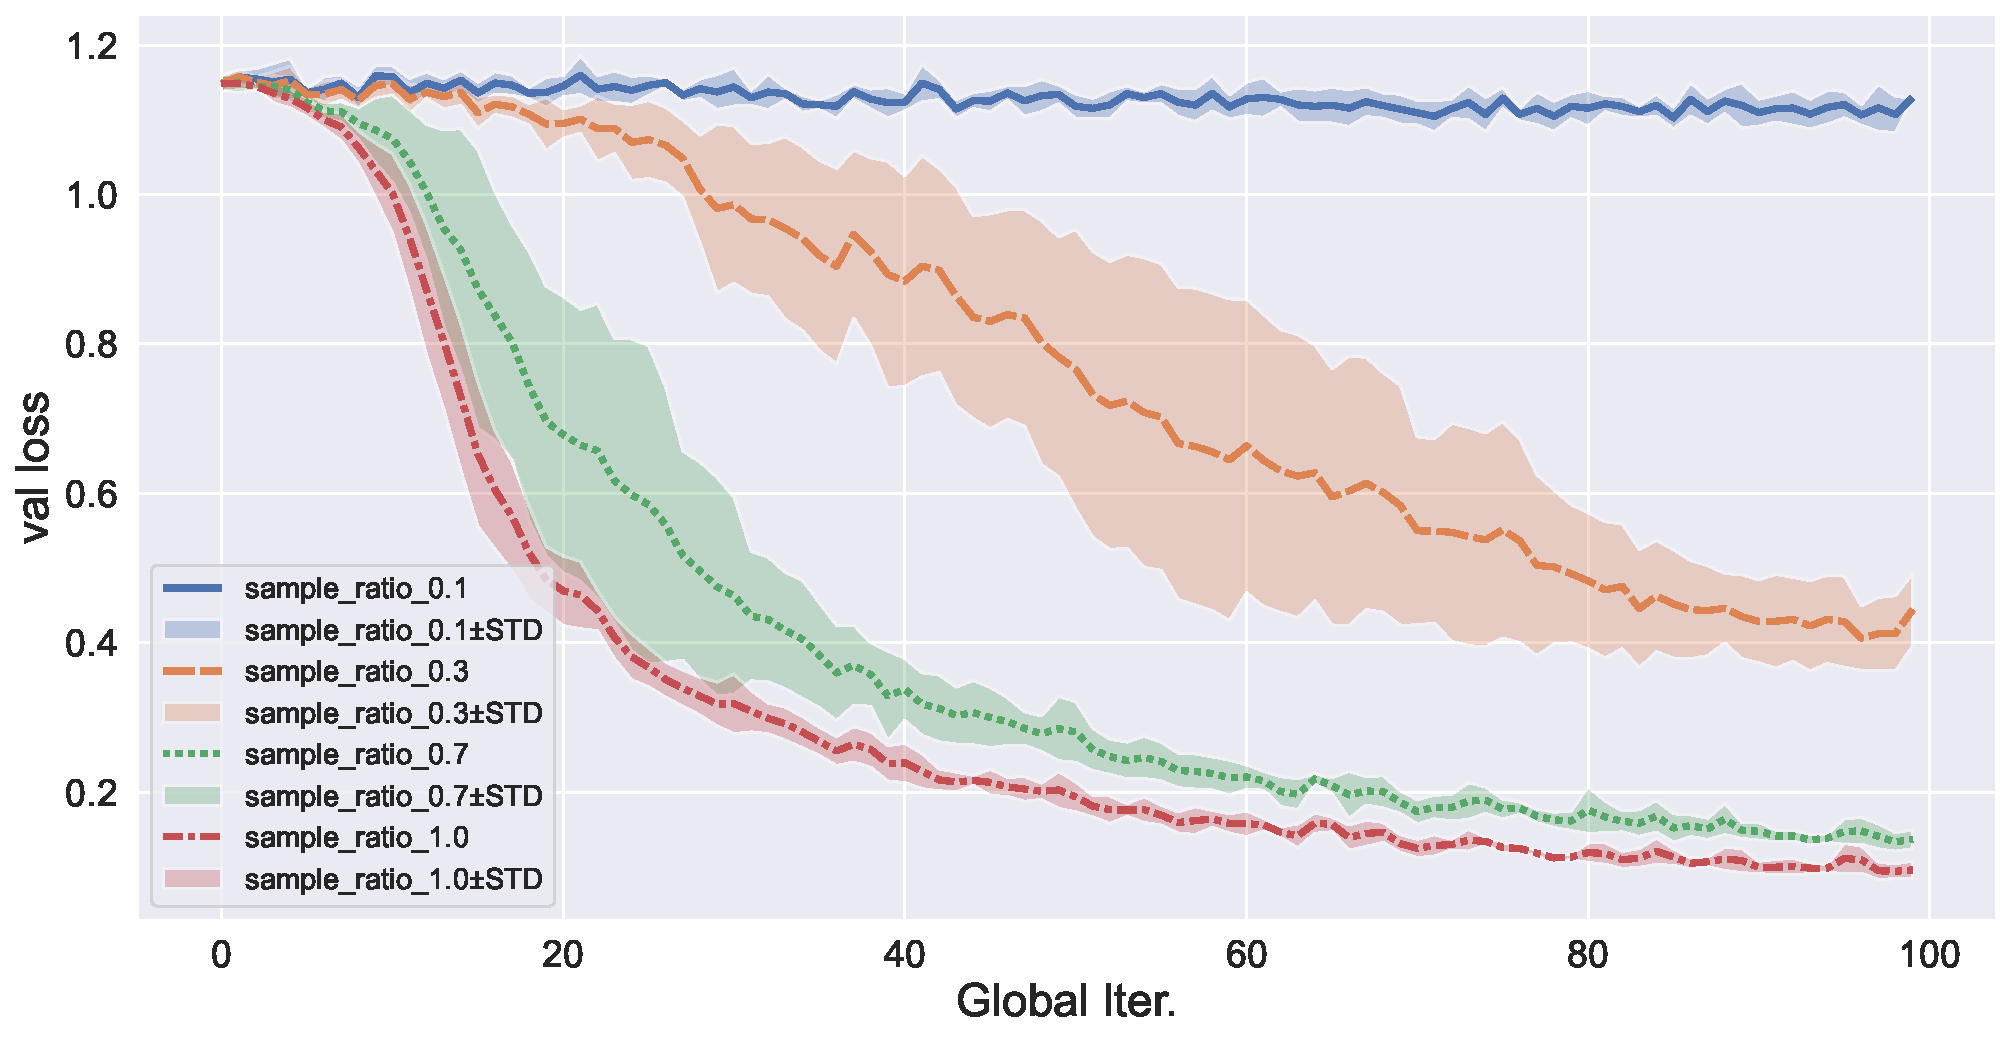
\includegraphics[width=.95\linewidth]{figures/proxskip-compare-sample-ratio-val-loss.pdf}
  \caption{\texttt{ProxSkip}算法在不同的子节点训练参与率下测试集上损失曲线}
  \label{fig:proxskip-compare-sample-ratio-val-loss}
\end{subfigure}
\begin{subfigure}{.5\textwidth}
  \centering
  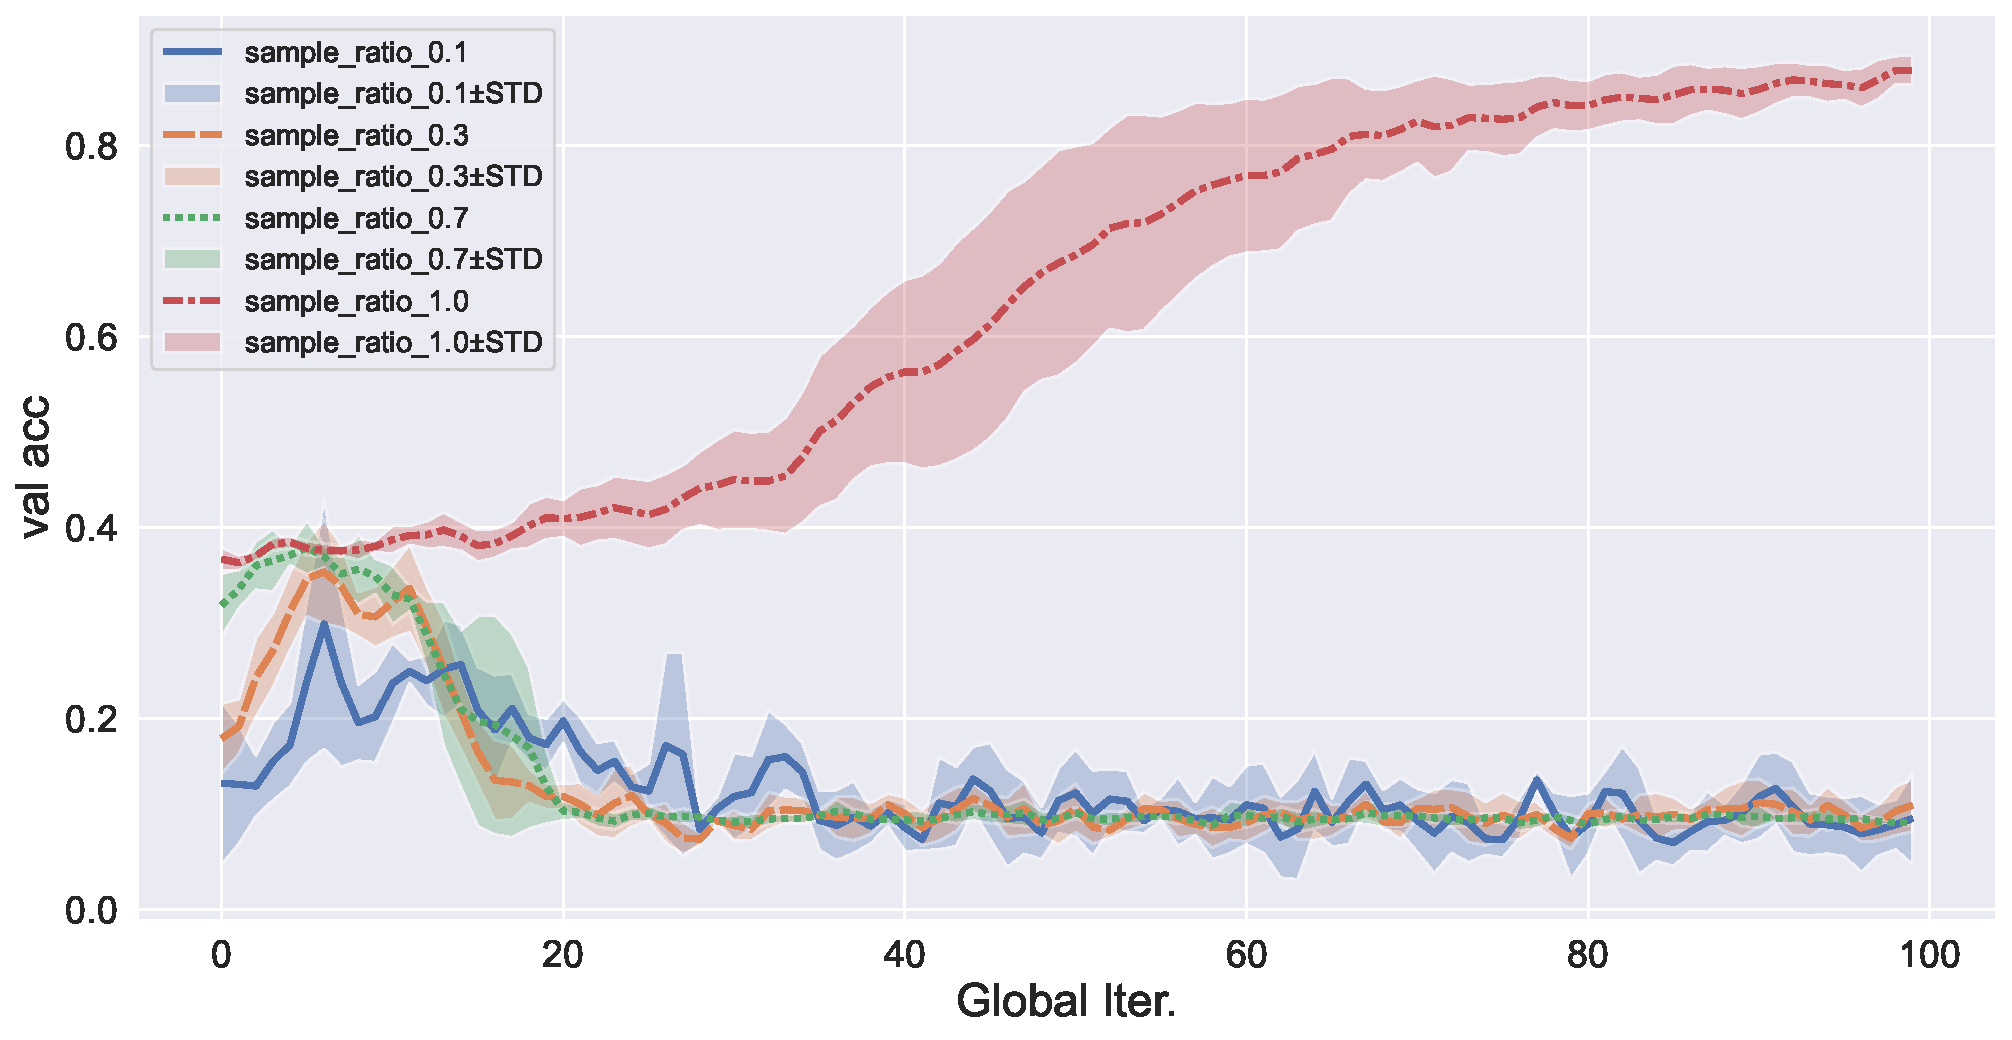
\includegraphics[width=.95\linewidth]{figures/fedsplit-compare-sample-ratio-val-acc.pdf}
  \caption{\texttt{FedSplit}算法在不同的子节点训练参与率下测试集上准确率曲线}
  \label{fig:fedsplit-compare-sample-ratio-val-acc}
\end{subfigure}%
\begin{subfigure}{.5\textwidth}
  \centering
  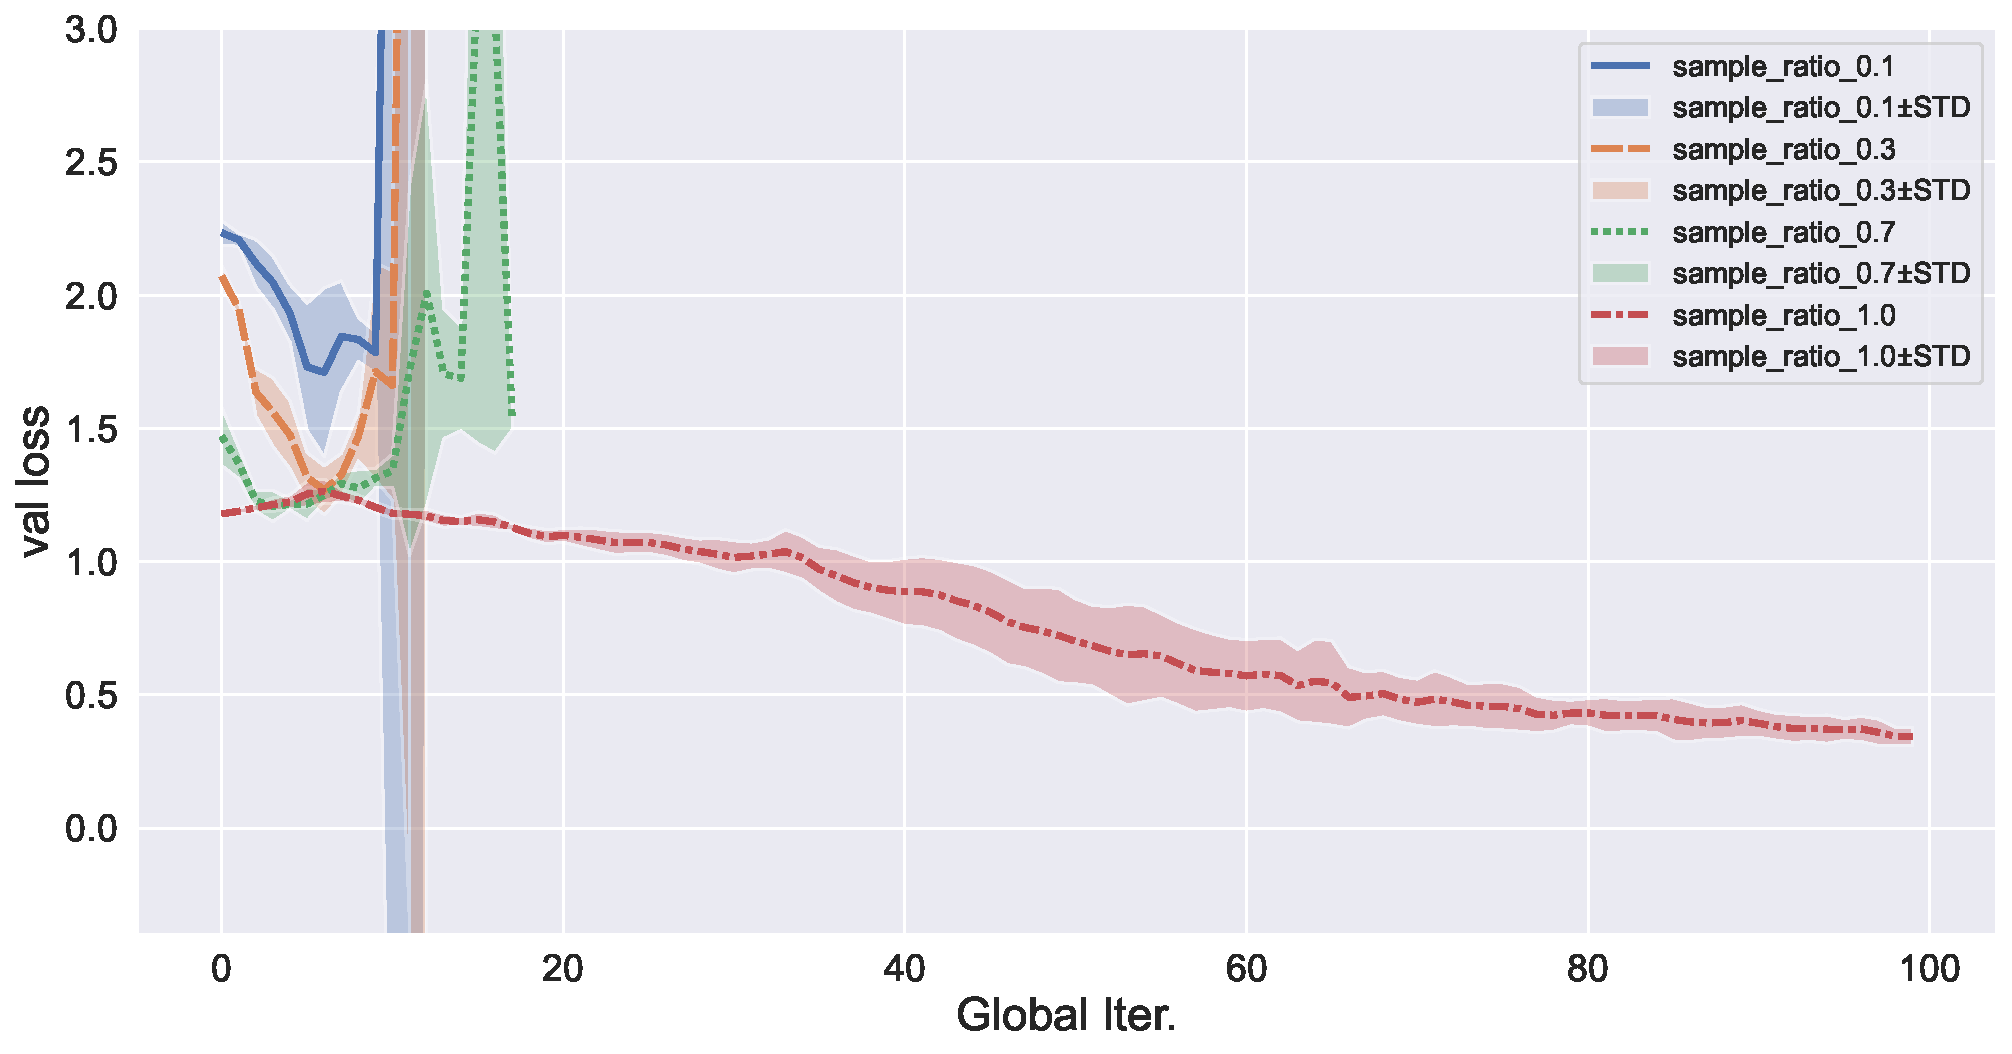
\includegraphics[width=.95\linewidth]{figures/fedsplit-compare-sample-ratio-val-loss.pdf}
  \caption{\texttt{FedSplit}算法在不同的子节点训练参与率下测试集上损失曲线}
  \label{fig:fedsplit-compare-sample-ratio-val-loss}
\end{subfigure}
\begin{subfigure}{.5\textwidth}
  \centering
  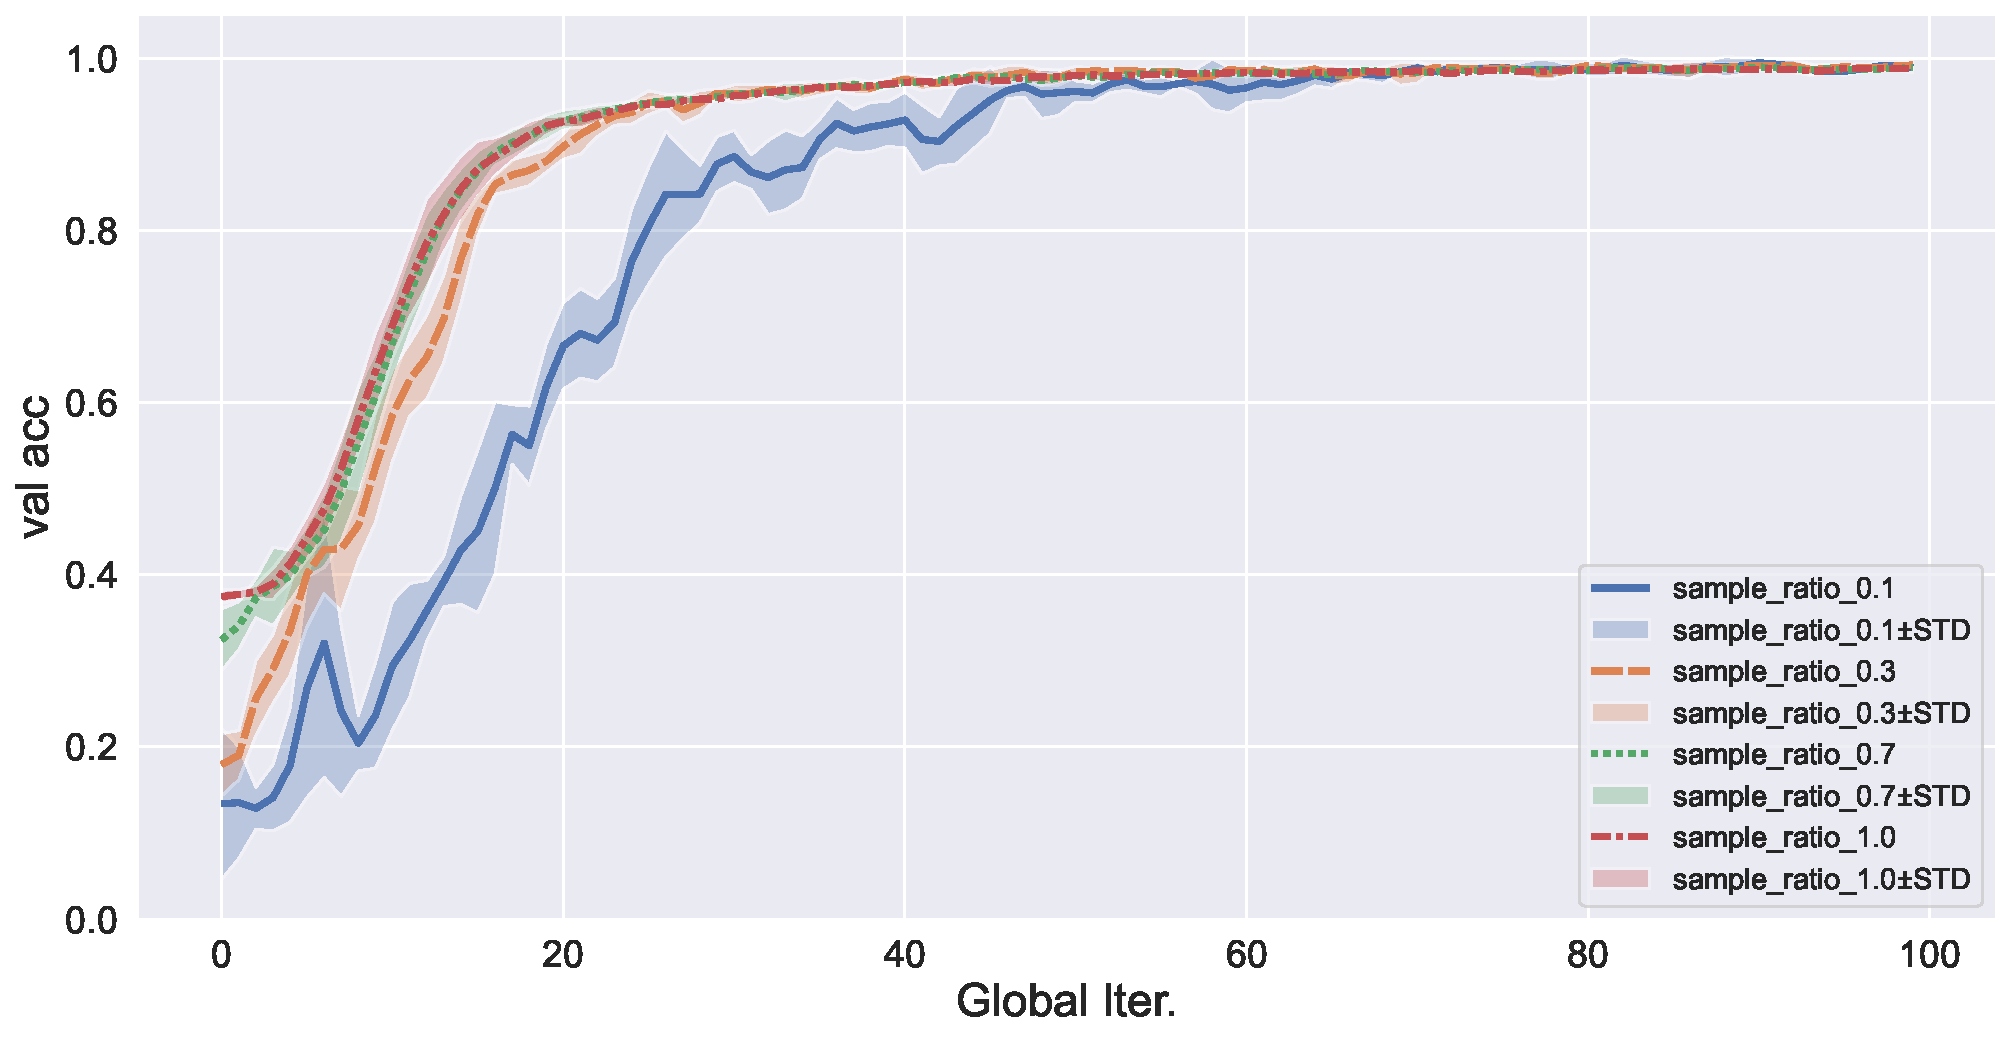
\includegraphics[width=.95\linewidth]{figures/ifca-compare-sample-ratio-val-acc.pdf}
  \caption{\texttt{IFCA}算法在不同的子节点训练参与率下测试集上准确率曲线}
  \label{fig:ifca-compare-sample-ratio-val-acc}
\end{subfigure}%
\begin{subfigure}{.5\textwidth}
  \centering
  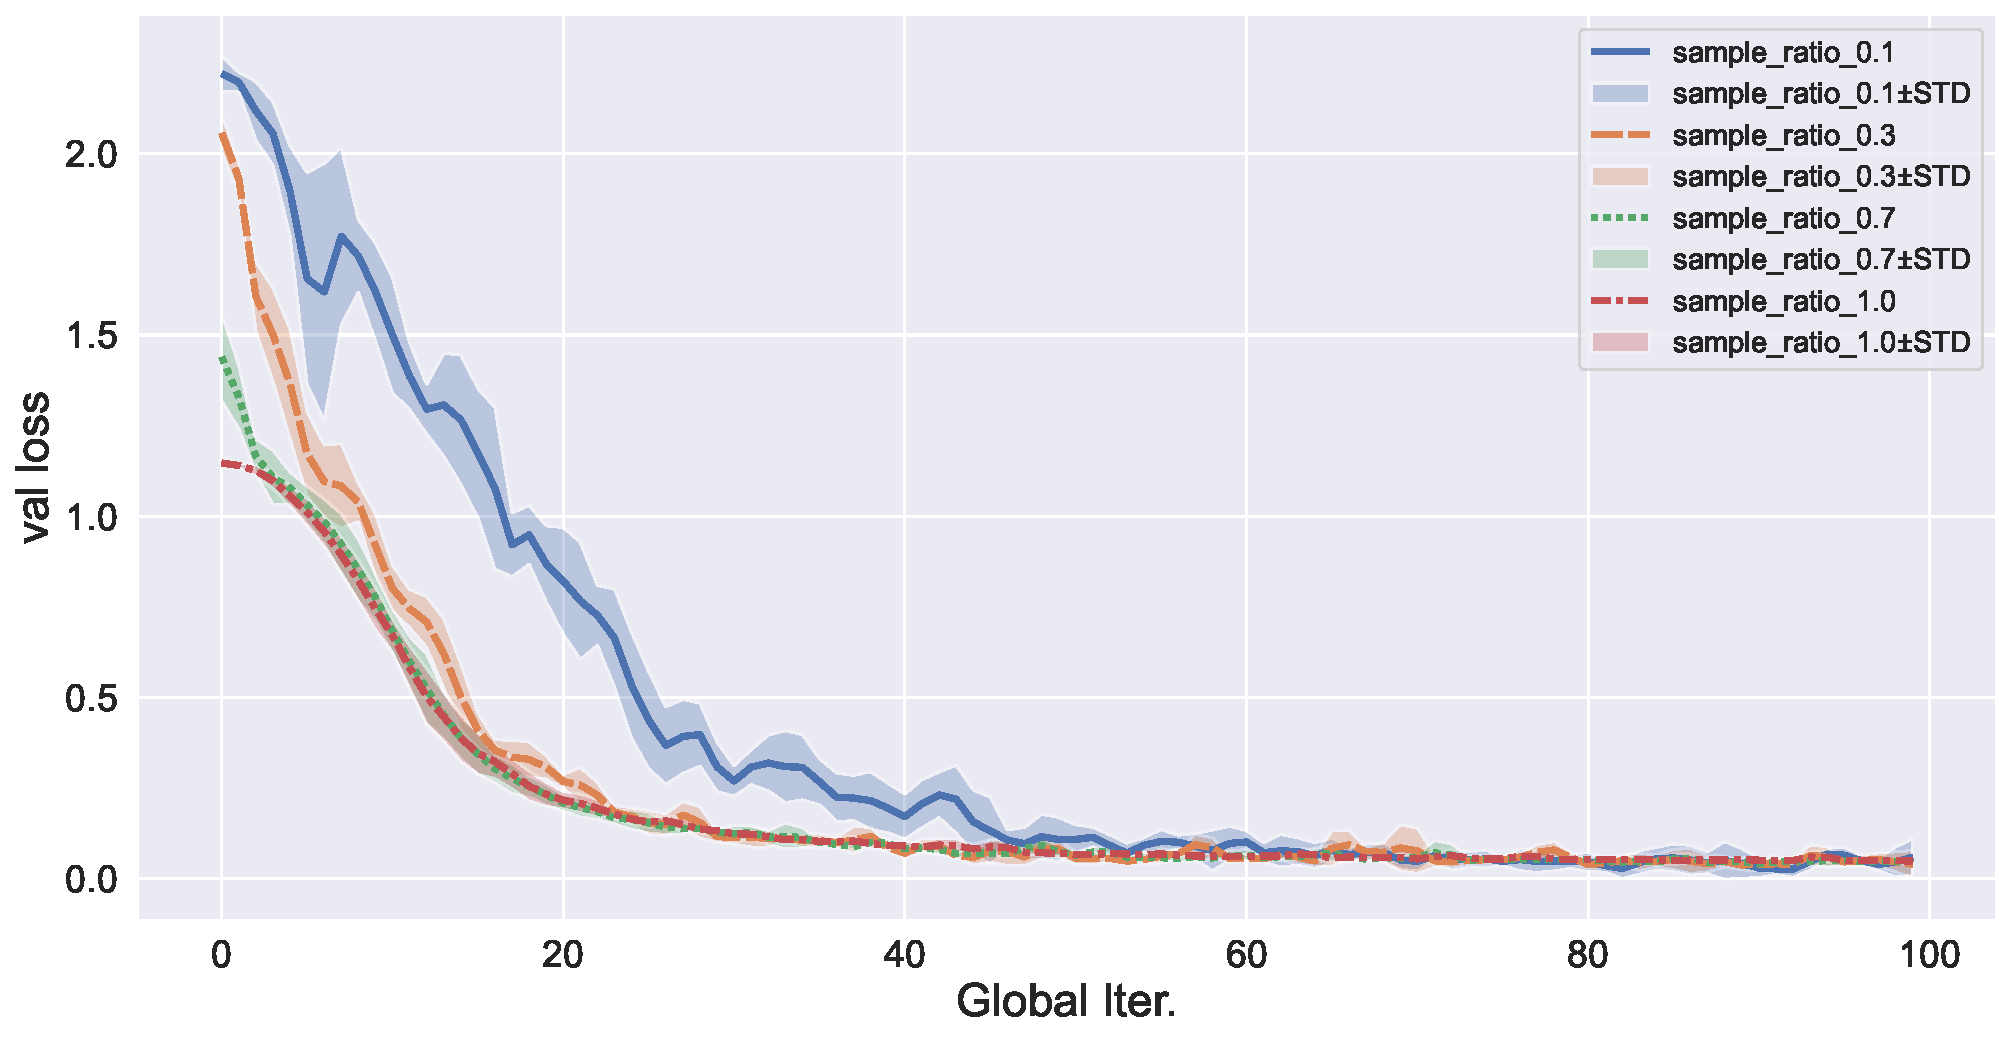
\includegraphics[width=.95\linewidth]{figures/ifca-compare-sample-ratio-val-loss.pdf}
  \caption{\texttt{IFCA}算法在不同的子节点训练参与率下测试集上损失曲线}
  \label{fig:ifca-compare-sample-ratio-val-loss}
\end{subfigure}
\caption{四种联邦学习算法在子节点训练参与率分别为$10\%, 30\%, 70\%, 100\%$下,在数据集\texttt{FedProxFEMNIST}的测试集上的准确率曲线以及损失曲线的对比。图中的sample\_ratio指的是子节点训练参与率。}
\label{fig:compare-sample-ratio}
\end{figure}

可以看到,当子节点训练参与率比较低的时候,联邦临近算法\texttt{FedProx} (子节点训练参与率在$10\%, 30\%$时) 准确率以及损失曲线波动比较大,收敛较慢;跳步算法\texttt{ProxSkip} (子节点训练参与率在$30\%, 70\%$时) 关于随机数种子的选取波动比较大 (图\ref{fig:proxskip-compare-sample-ratio-val-acc}~以及图\ref{fig:proxskip-compare-sample-ratio-val-loss}~中相应的表示使用不同随机数种子得到结果标准差的阴影面积比较大),这也是一个有趣的现象。对于联邦分裂算法\texttt{FedSplit}来说,当子节点训练参与率不足$100\%$时,损失函数的值在前20轮之内就发散到了无穷 (准确来说是超过了32位浮点数的表示范围),其可能的原因是发生了梯度或者是参数爆炸。这是值得继续深入研究的现象。
